\documentclass[12pt]{article}
\usepackage[left=1cm, right=1cm, top=2cm,bottom=1.5cm]{geometry} 

\usepackage[parfill]{parskip}
\usepackage[utf8]{inputenc}
\usepackage[T2A]{fontenc}
\usepackage[russian]{babel}
\usepackage{enumitem}
\usepackage[normalem]{ulem}
\usepackage{amsfonts, amsmath, amsthm, amssymb, mathtools}

\usepackage{fancyhdr}
\pagestyle{fancy}
\renewcommand{\headrulewidth}{1.5pt}
\renewcommand{\footrulewidth}{1pt}

\usepackage{graphicx}
\usepackage[figurename=Рис.]{caption}
\usepackage{subcaption}
\usepackage{float}

%%Наименование папки откуда забирать изображения
\graphicspath{ {./images/} }

%%Изменение формата для ввода доказательства
\renewcommand{\proofname}{$\square$  \nopunct}
\renewcommand\qedsymbol{$\blacksquare$}

\addto\captionsrussian{%
	\renewcommand{\proofname}{$\square$ \nopunct}%
}
%% Римские цифры
\newcommand{\RN}[1]{%
	\textup{\uppercase\expandafter{\romannumeral#1}}%
}

%% Для удобства записи
\newcommand{\MR}{\mathbb{R}}
\newcommand{\MQ}{\mathbb{Q}}
\newcommand{\MI}{\mathrm{I}}
\newcommand{\MJ}{\mathrm{J}}
\newcommand{\VN}{\varnothing}

\theoremstyle{definition}
\newtheorem{defn}{Опр:}
\newtheorem{rem}{Rm:}
\newtheorem{prop}{Утв.}
\newtheorem{exrc}{Упр.}
\newtheorem{lemma}{Лемма}
\newtheorem{theorem}{Теорема}
\newtheorem{corollary}{Следствие}

\newenvironment{cusdefn}[1]
{\renewcommand\thedefn{#1}\defn}
{\enddefn}



\DeclareRobustCommand{\divby}{%
	\mathrel{\text{\vbox{\baselineskip.65ex\lineskiplimit0pt\hbox{.}\hbox{.}\hbox{.}}}}%
}
\DeclareMathSymbol{\shortminus}{\mathbin}{AMSa}{"39}

\newcommand{\smallerrel}[1]{\mathrel{\mathpalette\smallerrelaux{#1}}}
\newcommand{\smallerrelaux}[2]{\raisebox{.1ex}{\scalebox{.75}{$#1#2$}}}

\newcommand{\smallin}{\smallerrel{\in}}
\newcommand{\smallnotin}{\smallerrel{\notin}}

\newcommand*{\medcap}{\mathbin{\scalebox{1.25}{\ensuremath{\cap}}}}%
\newcommand*{\medcup}{\mathbin{\scalebox{1.25}{\ensuremath{\cup}}}}%

\begin{document}
\lhead{Математический анализ - I}
\chead{Шапошников С.В.}
\rhead{Лекция - 19}

\section*{Свойства непрерывных функций на промежутках}

\begin{defn}
	Множество $\MI \subset \MR$ называется \uwave{промежутком}, если из того, что $x_1, x_2 \in \MI, \, x_1 \leq x_2 \Rightarrow [x_1,x_2] \subset \MI$.
\end{defn}

\textbf{Примеры}: $\MR, \, \VN$, точка, отрезок, полуинтервал - промежутки.

\begin{prop}
	Если $\MI$ - промежуток, то $\MI$ - это интервал или отрезок или полуинтервал (допускаются бесконечные концы).
\end{prop}

\begin{proof}
	Пусть $\MI \neq \VN$ и ограничен, по принципу полноты Вейрштрасса $\exists \, B = \sup{\MI}, \, A = \inf{\MI}$. Очевидно, что $\MI \subset [A,B]$. Покажем, что интервал $(A,B) \subset \MI$. \\
	Если $(A,B) = \VN$, то $A = B$ и множество $\MI$ - просто одна точка $= \{A\}$.\\
	Пусть $x \in (A,B) \Rightarrow A < x < B \Rightarrow x > A \Rightarrow x$ - не является нижней гранью $\MI \Rightarrow \exists \, x_1 \in \MI \colon x_1 < x$. Аналогично, $x < B \Rightarrow x$ - не является верхней гранью  $\MI \Rightarrow \exists \, x_2 \in \MI \colon x < x_2$. \\
	Получаем, что $x \in [x_1,x_2] \subset \MI$ - по определению промежутка $\Rightarrow x \in \MI$. Таким образом $\forall x \in (A,B) \Rightarrow$ $\Rightarrow x \in \MI \Rightarrow (A,B) \subset \MI$.
\end{proof}

\begin{exrc}
	Разобрать случай, когда $\MI$ не является ограниченным множеством.
\end{exrc}
\begin{proof}
	Пусть $\MI \neq \VN$ и не ограничен снизу и сверху. Очевидно, что $\MI \subset \MR$. 
	$\forall x \in \MR, \exists \, x_1, x_2 \in \MI \colon x \in [x_1,x_2] \Rightarrow x \in \MI \Rightarrow \MR \subset \MI \Rightarrow \MI = \MR$.
	
	Пусть $\MI \neq \VN$ и не ограничен сверху, но ограничен снизу $\Rightarrow$ по принципу полноты Вейрштрасса $\exists \, A = \inf{\MI}$. Очевидно, что $\MI \subset [A,+\infty)$. Покажем, что полуинтервал $(A,+\infty) \subset \MI$. Пусть $x \in (A,+\infty) \Rightarrow A < x  \Rightarrow x > A \Rightarrow x$ - не является нижней гранью $\MI \Rightarrow \exists \, x_1 \in \MI \colon x_1 < x$. Так как $\MI$ не ограничен сверху, то $\exists \, x_2 \in \MI \colon x < x_2$. Получаем, что $x \in [x_1,x_2] \subset \MI$ - по определению промежутка $\Rightarrow x \in \MI$. Таким образом $\forall x \in (A,+\infty) \Rightarrow x \in \MI \Rightarrow (A,+\infty) \subset \MI$.
\end{proof}

\begin{corollary}\textbf{(Из теоремы о промежуточном значении)}
	Если $\MI \neq \VN$ - промежуток и $f \colon \MI \to \MR$ - непрерывная функция, то образ $f(\MI) = \{\, y \colon \exists \, x \in \MI, f(x) = y \,\}$ является промежутком.
\end{corollary}

\begin{proof}
	Если $\MI$ - это точка, то утверждение очевидно. Пусть в $\MI$ более одной точки. Надо проверить: \\
	$\forall y_1, y_2 \in f(\MI), \, y_1 \leq y_2$ верно, что $[y_1, y_2] \subset f(\MI)$. 
	Возьмем $x_1 \in \MI \colon f(x_1) = y_1$, $x_2 \in \MI \colon f(x_2) = y_2$. Пусть $x_1 \leq x_2$. Если $x_1 = x_2 \Rightarrow y_1 = y_2$ и все доказано. 
	
	Если $x_1 < x_2 \Rightarrow [x_1, x_2] \subset \MI$. Поскольку $f$ - непрерывна на $[x_1, x_2] \Rightarrow$ по теореме о промежуточном значении $\forall y \in [y_1, y_2], \, \exists \, x \in [x_1, x_2] \colon y = f(x) \Rightarrow [y_1, y_2] \subset f(\MI)$.
\end{proof}

\begin{rem}
	Если $f\colon \MR \to \MR$ всякий промежуток отображает в промежуток, то это не означает, что $f$ - непрерывная функция. 
\end{rem}

\textbf{Пример}: $$ f(x) = \begin{cases} 
	\sin{\frac{1}{x}}, & x \neq 0\\
	0, & x = 0
\end{cases}
$$

Данная функция определена на всей числовой прямой и отображает промежутки в промежутки. 

Если $0$ попадет в промежуток, то образом будет отрезок $[-1,1]$. Но при этом функция не является непрерывной.

\newpage 

\begin{theorem}
	Если $f$ - монотонна на промежутке $\MI \neq \VN$ и $f(\MI)$ - промежуток, то $f$ - непрерывна на $\MI$.
\end{theorem}

Если функция монотонна (пусть она не убывает), тогда она имеет пределы слева, справа и какое-то значение в точке $x_0$.
\begin{figure}[H]
	\centering
	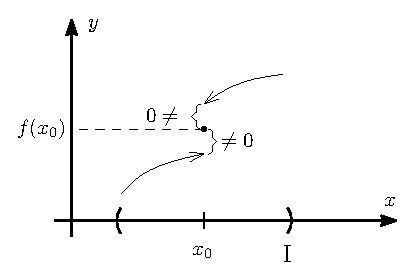
\includegraphics[width=0.33\textwidth]{19_1.eps}
	\caption{Монотонная функция не убывает на $\MI$, имеет пределы слева и справа.}
	\label{19_1}
\end{figure}

 Если есть разрыв в этой точке, то хотя бы с одной из сторон будет ненулевое расстояние между значением в точке и односторонним пределом. Пусть предел слева $=A$ отличается от значения в $x_0 \colon A \neq f(x_0)$. Все точки левее $x_0$ будут меньше предела слева. Все точки правее $x_0$ будут больше или равны $f(x_0)$.

\begin{figure}[H]
	\begin{subfigure}[b]{0.5\textwidth}
		\centering
		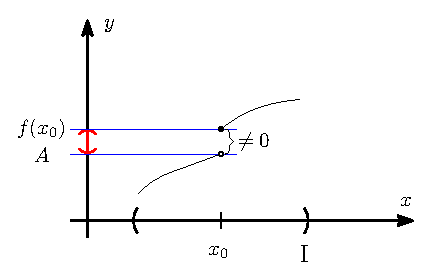
\includegraphics[width=0.85\textwidth]{19_2.eps}
		\caption{Предел слева $\neq f(x_0)$. Интервал $(A,f(x_0)) \not\subset f(\MI)$.}
		\label{19_2}
	\end{subfigure}%
	\begin{subfigure}[b]{0.5\textwidth}
		\centering
		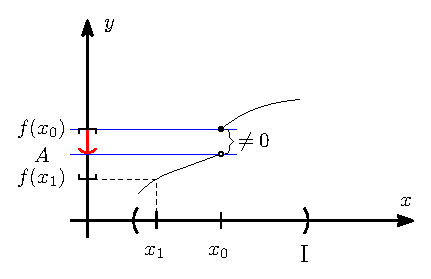
\includegraphics[width=0.85\textwidth]{19_3.eps}
		\caption{$x_1 < x_0,\,[f(x_1),f(x_0)] \subset f(\MI)$.}
		\label{19_3}
	\end{subfigure}
	\caption{Непрерывность монотонной функции отображающей промежутки в промежутки.}
\end{figure}

В этом случае, интервала $(A,f(x_0))$ точно нет в $f(\MI)$. Возьмем точку $x_1 < x_0 \Rightarrow [f(x_1),f(x_0)] \subset f(\MI)$, так как образ по условию это промежуток. Таким образом, у монотонной функции разрывы выбивают в области значения дырки, что запрещено тем, что образ это промежуток.
 
\begin{proof}
	(От противного) Пусть $x_0$ - внутренняя точка $\MI$ (если $x_0$ - граничная точка, то будет аналогично). Пусть $f$ - не убывает, тогда 
	$$\exists \! \lim\limits_{x \to x_0-}f(x) = \sup\limits_{x < x_0}{f} = A, \, \exists \! \lim\limits_{x \to x_0+}f(x) = \inf\limits_{x > x_0}{f} = B$$
	Если $x_0$ - точка разрыва $f$, то хотя бы одно из неравенств $A < f(x_0) \vee f(x_0) < B$ - верно, иначе это была бы точка непрерывности. Пусть $A < f(x_0)$, тогда $\forall x < x_0, \, f(x) \leq A, \, \forall x \geq x_0, \, f(x) \geq f(x_0)$ и $(A, f(x_0)) \cap f(\MI) = \VN$. С другой стороны $\forall x_1 < x_0, \, [f(x_1), f(x_0)] \subset f(\MI)$ и $(A, f(x_0)) \subset [f(x_1),f(x_0)]$, так как $f(x_1) \leq A \Rightarrow$ получили противоречие.	
\end{proof}

\begin{exrc}
	Доказать в случае, если $x_0$ - граничная точка.
\end{exrc}
\begin{proof}
	(От противного) Пусть $x_0$ - граничная точка $\MI$ справа. Пусть $f$ - не убывает, тогда 
	$$\exists \! \lim\limits_{x \to x_0-}f(x) = \sup\limits_{x < x_0}{f} = A$$
	Если $x_0$ - точка разрыва $f$, то $A < f(x_0)$, иначе это была бы точка непрерывности. В этом случае $\forall x < x_0, \, f(x) \leq A$ и $(A, f(x_0)) \cap f(\MI) = \VN$. С другой стороны $\forall x_1 < x_0, \, [f(x_1), f(x_0)] \subset f(\MI)$ и $(A, f(x_0)) \subset [f(x_1),f(x_0)]$, так как $f(x_1) \leq A \Rightarrow$ получили противоречие. Аналогично для граничной точки слева.
\end{proof}

\begin{theorem}\textbf{(Об обратной функции)}
	Пусть $\MI \neq \VN$ промежуток и $f \colon \MI \to \MR$ - непрерывная, строго монотонная функция. Тогда 
	\begin{enumerate}[label={\arabic*)}]
		\item $f(\MI) = \MJ = \{\, y \colon \exists \, x \in \MI, f(x) = y \,\}$ - непустой промежуток;
		\item $f\colon \MI \to \MJ$ - биекция;
		\item $f^{-1} \colon \MJ \to \MI$ - строго монотонна и непрерывна;
	\end{enumerate}
\end{theorem}

\begin{proof}\hfill
	\begin{enumerate}[label={\arabic*)}]
		\item При непрерывном отображении, образ промежутка это промежуток;
		\item Из строгой монотонности следует, что функция инъективна. Отображение на свой образ всегда сюръективно. Поэтому функция $f$ - биекция;
		\item Если $f^{-1}$ - строго монотонна на промежутке $\MJ$, то $f^{-1}$ - непрерывна на нем, так как образ промежутка - промежуток;
	\end{enumerate}
	Поэтому достаточно проверить, что функция $f^{-1}$ - строго монотонна. Возьмем $y_1 < y_2 \Rightarrow$ сравним $f^{-1}(y_1)$ и $f^{-1}(y_2)$. Пусть для определенности $f$ - возрастает $\Rightarrow x_1 = f^{-1}(y_1), \, x_2 = f^{-1}(y_2)$. $x_1 \neq x_2$, иначе $y_1 = f(x_1) = f(x_2) = y_2$. Пусть $x_1 > x_2 \Rightarrow y_1 = f(x_1) > f(x_2) = y_2$, но по условию $y_1 < y_2 \Rightarrow$ противоречие $\Rightarrow x_1 < x_2 \Rightarrow f^{-1}(y_1) < f^{-1}(y_2)$.
\end{proof}

\begin{rem}
	Направление монотонности у $f^{-1}$ будет такое же, как и у $f$ (по доказательству теоремы).
\end{rem}

\textbf{Пример}: $y = x^{2n+1}, \, n \in \mathbb{N}$; \\
$f$ всюду определена на $\MR$. $f$ - непрерывная функция $\Rightarrow$ её область значений это промежуток, он не ограничен сверху и снизу: $m^{2n+1} \xrightarrow[m\to \infty]{} +\infty, \, (-m)^{2n+1} \xrightarrow[m\to \infty]{} -\infty \Rightarrow$ область значений $\MR$. Эта функция возрастает $\Rightarrow$ по теореме об обратной функции $\exists \, f^{-1} \colon \MR \to \MR$ - непрерывна и возрастает. $$f^{-1}(y) = y^{\frac{1}{2n+1}} = \sqrt[\leftroot{-2}\uproot{2}{2n+1}]{y}$$

\textbf{Пример}: $y = x^{2n}, \, n \in \mathbb{N}$; \\
$f$ всюду определена на $\MR$. $f$ - непрерывная функция $\Rightarrow$ её область значений это промежуток, он не ограничен сверху: $m^{2n} \xrightarrow[m\to \infty]{} +\infty \Rightarrow$ область значений $[0, +\infty)$. Эта функция имеет два промежутка монотонности. Выберем $[0, +\infty)$, на нем она возрастает и отображает его на $[0, +\infty) \Rightarrow$ по теореме об обратной функции $\exists \, f^{-1} \colon [0, +\infty) \to [0, +\infty)$ - непрерывна и возрастает. $$f^{-1}(y) = y^{\frac{1}{2n}} = \sqrt[\leftroot{-2}\uproot{2}{2n}]{y}$$

\begin{rem}
	Аналогично строятся другие обратные функции: берется промежуток, где функция непрерывна и строго монотонна и применяется теорема об обратной функции.
\end{rem}
\newpage

\section*{Построение функции $a^x$}
Пусть $a > 1$. В школе: 
\begin{enumerate}
	\item $a^n = \underbrace{a\cdot \dotsc \cdot a}_{n}$;
	\item $a^0 = a^{1-1} = \dfrac{a}{a} = 1$;
	\item $a^{-n} = (a^n)^{-1} = \dfrac{1}{a^{n}}$;
	\item $a^{\frac{p}{q}} = \Big( a^{\frac{1}{q}} \Big)^p$ определили выше функции в степени $\frac{1}{n}, \, n \in \mathbb{N}$;
\end{enumerate}

Таким образом, возникает функция $y = a^x, \, x \in \MQ$. У нее есть следующие свойства:
\begin{enumerate}
	\item $a^0 = 1$;
	\item $a^{x+ y} = a^xa^y$;
	\item $x < y \Rightarrow a^x < a^y$ (строгая монотонность);
	\item $a^n \to +\infty, \, a^{-n} \to 0$ (доказывается так, например: $a^n = (1 + a -1)^n \geq 1 + n(a-1)$);
\end{enumerate}

Как определить $a^x$ для $x \notin \MQ$? 

\uline{\textbf{Идея}}: возьмем $r_n \in \MQ \colon r_n \to x, \, a^x = \lim\limits_{n \to \infty} a^{r_n}$. Будут ли эти числа сходится? Почему они будут сходится к одному и тому же? $r_n \to r \in \MQ \Rightarrow a^r = \lim\limits_{n \to \infty} a^{r_n}$?

\begin{prop}
	Предположим, что $f$ определена на $\MQ \cap [a,b]$ и удовлетворяет условию: 
	$$|f(x) - f(y)| \leq C |x-y|, \, \forall x,y \in \MQ \cap [a,b]$$ 
	Тогда $\exists! \, \tilde{f}$ - непрерывная функция на $[a,b] \colon f = \tilde{f}$ на $\MQ \cap [a,b]$.
\end{prop}

\begin{proof}
	Пусть $r_n \to x, \, r_n \in \MQ$, положим, что $\tilde{f}(x) = \lim\limits_{n\to \infty} f(r_n)$. Проверим, что этот предел существует, не зависит от выбора $r_n$ и совпадает со значением функции $f$, если приближаемся к рациональной точке.
	
	\uwave{Существование}: Возьмем $r_n, r_m$, по условию $|f(r_n) - f(r_m)| \leq C|r_n - r_m|$, $r_n$ - сходится $\Rightarrow$ последовательность фундаментальна $\Rightarrow$ выполняется условие Коши $\Rightarrow \forall \varepsilon > 0, \exists \, N \colon \forall n, m > N \Rightarrow |r_n -r_m| < \varepsilon \Rightarrow |f(r_n) - f(r_m)| < C \varepsilon$, то есть $f(r_n)$ - фундаментальна и значит $\exists \lim\limits_{n \to \infty}f(r_n)$.
	
	\uwave{Независимость от выбора $r_n$}: Пусть $r_n \to x \wedge s_n \to x \Rightarrow |f(r_n) - f(s_n)| \leq C|r_n - s_n| \to 0 \Rightarrow$ \\
	$\Rightarrow \lim\limits_{n \to \infty}f(r_n) =  \lim\limits_{n \to \infty}f(s_n)$.
	
	\uwave{Совпадение в рациональных точках}: Если $x \in \MQ \Rightarrow r_n \equiv x \Rightarrow \lim\limits_{n \to \infty}f(r_n) = f(x)$. 
	
	Следовательно, такое определение $\tilde{f}(x) = \lim\limits_{n\to \infty} f(r_n)$ - корректно и $\tilde{f} = f$ на $\MQ$. 
	
	Возьмем $x,y$ и возьмем $r_n \to x, \, s_n \to y$. Знаем, что $|f(r_n) - f(s_n)| \leq C|r_n - s_n| \Rightarrow$ \\ 
	$\Rightarrow |f(r_n) - f(s_n)|\to |\tilde{f}(x) - \tilde{f}(y)|, \, C|r_n -s_n| \to C|x-y| \Rightarrow |\tilde{f}(x) - \tilde{f}(y)| \leq C|x-y| \Rightarrow \tilde{f}$ - непрерывна.
	
	\uwave{Единственность}: Пусть есть две $\tilde{f}_1, \tilde{f}_2$ - непрерывные функции: $\tilde{f}_1 = f = \tilde{f}_2$ на $\MQ \Rightarrow \tilde{f}_1(x) = f = \tilde{f}_2(x), \, \forall x$ по непрерывности: $r_n \in Q, \, r_n \to x, \, \tilde{f}_1(r_n) \to \tilde{f}_1(x), \, \tilde{f}_2(r_n) \to \tilde{f}_2(x)$, но $\tilde{f}_1(r_n) =  \tilde{f}_2(r_n) \Rightarrow$ равны их пределы $\Rightarrow \tilde{f}_1(x) = \tilde{f}_2(x)$.
\end{proof}

\begin{prop}
	 $\forall\, [-N,N], \exists \, C(N) \colon |a^x - a^y| \leq C(N)|x-y|, \forall x,y \in \MQ \cap [-N,N]$.
\end{prop}

\begin{proof}\hfill\\
	$(1)$ $1 < a^\frac{1}{n} =(1 + a - 1)^\frac{1}{n} \leq 1 + \dfrac{a - 1}{n}$ (нер-во Бернулли) $\Rightarrow a^\frac{1}{n} - 1 \leq \dfrac{a - 1}{n}$. Пусть $0 < x \leq 1, \, x \in \MQ \Rightarrow$ \\
	$$\dfrac{1}{n+1} < x \leq \dfrac{1}{n} \Rightarrow a^x - 1 \leq a^\frac{1}{n} -1 \leq \dfrac{a-1}{n} = (a-1){\cdot}\dfrac{n+1}{n}{\cdot}\dfrac{1}{n+1} \leq 2 (a-1) x, \, \forall x \in (0,1] \cap \MQ$$ 
	$\Rightarrow a^x - 1 \leq 2(a-1)x$;
	
	$(2)$ $\forall x,y, \in [-N, N] \cap \MQ$. Если $x = y \Rightarrow$ утверждение очевидно: $0 \leq 0$. Пусть $x > y \Rightarrow$ 
	$$|a^x - a^y| = a^y(a^{x-y} - 1) \leq a^N(a^{x-y} -1)$$ 
	так как функция монотонная. Если $0 < x - y \leq 1 \Rightarrow |a^x - a^y| \leq a^N 2(a-1)(x-y)$. Если $1 < x-y \Rightarrow |a^x - a^y| \leq a^{3N}(x-y)$, так как $x,y \in [-N,N] \Rightarrow \max\{x-y\} = N - (-N) = 2N$. 
	
	$(3)$ Таким образом $C(N) = \max\{a^N2(a-1), a^{3N}\}$;

\end{proof}

\end{document}